% !TEX encoding = UTF-8
% !TEX TS-program = pdflatex
% !TEX root = ../tesi.tex

%**************************************************************
\chapter{Experimental setup}
\label{cap:chapter3}
%**************************************************************

%**************************************************************

\section{Development environment}

To ensure reproducibility of our experiments, this section details the hardware architecture, core software dependencies, and the key modeling simplifications adopted throughout this work. Our primary simplification is the reduction of the search space to a single dimension, fixing the elevation angle at $\theta = 0^\circ$ and optimizing exclusively over the azimuth.

\subsection{Programming language}

Given the field and scope of the problem, the Python programming language has been chosen because of the wealth of\gls{AI} research carried out in the language and the consequently established ecosystem of scientific libraries developed.  It is also a more well-know language in the scientific literature for future peer review and improvements.

\subsection{Development tools}

The choice of tool used to handle the python development environment was uv, a Python package and project manager. With respect to the classic approach of using pip with virtual environment and a requirements.txt file, uv enables the developer to have more granular control on the dependencies' versions. 


\begin{longtable}{@{}|l|p{7cm}|l|@{}}
\caption{Programming language \& Environment tools }
\label{tab:programming-environment}\\
\hline
\textbf{Component} & \textbf{Details} & \textbf{Version} \\
\hline
\endfirsthead

\multicolumn{3}{c}%
{{\tablename\ \thetable{} -- \textit{Continued from previous page}}} \\
\hline
\textbf{Component} & \textbf{Details} & \textbf{Version} \\
\hline
\endhead

\hline
\multicolumn{3}{r}{\textit{Continued on next page}} \\
\endfoot

\hline
\endlastfoot

Python & Main programming language for AI & ~=3.14.3 \\
\hline
uv & Fast Python package and project manager & 0.8.15 \\
\hline
ruff & Fast Python linter and code formatter & 0.15.6 \\
\end{longtable}
\newpage

\begin{longtable}{@{}|l|p{7cm}|l|@{}}
\caption{Python Libraries Used in the Project}
\label{tab:python-libraries}\\
\hline
\textbf{Library Name} & \textbf{Description} & \textbf{Version} \\
\hline
\endfirsthead

\multicolumn{3}{c}%
{{\tablename\ \thetable{} -- \textit{Continued from previous page}}} \\
\hline
\textbf{Library Name} & \textbf{Description} & \textbf{Version} \\
\hline
\endhead

\hline
\multicolumn{3}{r}{\textit{Continued on next page}} \\
\endfoot

\hline
\endlastfoot

gymnasium & Reinforcement learning environments & 1.2.3 \\
\hline
matplotlib & Plotting and visualization library & 3.10.8 \\
\hline
numpy & Numerical computing and array operations & 2.4.3 \\
\hline
scipy & Scientific computing and numerical algorithms & 1.17.1 \\
\hline
stable-baselines3 & Reinforcement learning algorithms & 2.7.1 \\
\hline
torch & Deep learning framework & 2.11.0 \\
\hline
triton & GPU programming language and compiler & 3.6.0 \\
\end{longtable}



\begin{longtable}{@{}|l|p{7cm}|l|@{}}
\caption{Hardware Used in the Project}
\label{tab:hardware-used}\\
\hline
\textbf{Component} & \textbf{Details} \\
\hline
\endfirsthead

\multicolumn{3}{c}%
{{\tablename\ \thetable{} -- \textit{Continued from previous page}}} \\
\hline
\textbf{Component} & \textbf{Details} \\
\hline
\endhead

\hline
\multicolumn{3}{r}{\textit{Continued on next page}} \\
\endfoot

\hline
\endlastfoot

CPU & Intel(R) Xeon(R) Gold 5418Y, CPU family: 6, Model: 143, Architecture: x86\_64 \\
\hline
GPU & Nvidia RTX 4090 \\
\end{longtable}

\section{Environment}
{\color{blue}I: Here you are explaining the principle of RL. You are not really describing your environment}
In this reinforcement-learning model, the agent is connected to its environment, and at each step of interaction the agent receives as input, \textit{i}, some indication of the current state, \textit{s}, of the environment; the agent then chooses an action, \textit{a}, to generate as output. The value of the action is calculated through a reward function, \textit{R}, and the behavior of the agent, \textit{B}, choosing actions that tend to increase the long-term sum of values \cite{kaelbling1996rl}. It learns over time by systematic trial and error, guided by an algorithm. 



\subsection{Training angles and sampling strategy}
{\color{blue}I: This first sentence is not clear to me}
In our\gls{ULA}-based DDM context, there are difficulties related to angle-dependent constraints and also sin-space sampling biases. 

\subsubsection{The Spatial Frequency Domain of a ULA}

The array response of a\gls{ULA} with $N$ elements and inter-element spacing $d$ is governed by the projection of the incoming wave vector onto the array axis. For an array oriented along the $y$-axis, with element positions $\mathbf{u}_n = [0,\, nd,\, 0]^\top$ for $n = 0, \ldots, N-1$, and a source at elevation $\theta = 0\degree $ and azimuth $\varphi$, the wave vector component along the array axis reduces to:
\begin{equation}
    k_y(\varphi) = \frac{2\pi}{\lambda}\sin\varphi
\end{equation}
The array manifold vector, the per-element phase accumulated by a plane wave arriving from $\varphi$, is therefore:
\begin{equation}
    \mathbf{v}(\varphi) = \left[1,\; e^{j\pi\sin\varphi},\; e^{j2\pi\sin\varphi},\; \ldots,\; e^{j(N-1)\pi\sin\varphi}\right]^\top
\end{equation}
where we have assumed $d = \lambda/2$. Given a steering vector $\mathbf{a} = [a_0, \ldots, a_{N-1}]^\top = [\alpha_n e^{j\psi_n}]$, the normalised array response is:
\begin{equation}
    f(\varphi) = \frac{1}{N}\mathbf{a}^H \mathbf{v}(\varphi) = \frac{1}{N}\sum_{n=0}^{N-1} \alpha_n\, e^{j(\pi\sin\varphi \cdot n - \psi_n)}
\end{equation}
A critical observation follows directly from this expression: $\varphi$ appears exclusively through $\sin\varphi$. Defining the direction cosine $u \triangleq \sin\varphi \in [-1, 1]$, the array response becomes a Fourier-like polynomial in $e^{j\pi u}$:
\begin{equation}
    f(u) = \frac{1}{N}\sum_{n=0}^{N-1} \alpha_n\, e^{j(\pi u \cdot n - \psi_n)}
\end{equation}
The array has no means of distinguishing between two directions that share the same value of $u$. Equivalently, all physics of the beamforming problem (gain, phase flatness, constraint satisfaction) is determined entirely by the spatial frequency $u$, not by the azimuth angle $\varphi$ per se.
\subsubsection{Angle-Dependent Constraint Difficulty}
\label{subsec:angle_dependant_constraint}
The\gls{DDM} validity constraint requires that, for a given target direction $\varphi^*$, the array response $f(\varphi)$ satisfies two conditions simultaneously over the angular support $[\varphi^* - \delta\varphi,\, \varphi^* + \delta\varphi]$ (with $\delta\varphi = 5\degree$ in the system under study):
\begin{align}
    \log_{10}|f(\varphi)| &\geq \varepsilon_a & &\text{(amplitude floor)}  \label{eq:ddm_amplitude} \\
    |\angle f(\varphi) - \angle f(\varphi^*)| &\leq \varepsilon_p & &\text{(phase flatness)} \label{eq:ddm_phase}
\end{align}
where $\varepsilon_p = 10\degree$ is the phase tolerance. Note that $\varepsilon_a$ is the raw base-10 logarithm of the normalised amplitude. The phase flatness condition is the binding constraint for secrecy: it forces the phase of the received signal to remain approximately constant within the legitimate receiver's angular neighbourhood while allowing it to vary freely, and ideally rapidly, outside. Because the array response depends only on $u = \sin\varphi$, the angular support maps to an interval in $u$-space of width:
\begin{equation}
    \Delta u(\varphi^*) = |\sin(\varphi^* + \delta\varphi) - \sin(\varphi^* - \delta\varphi)| = 2\cos\varphi^*\sin(\delta\varphi)
\end{equation}
This width is maximised at broadside and collapses toward zero at endfire, meaning that the feasible set of valid steering vectors is smallest at broadside. \figurename~\ref{fig:sampling_constraint_bandwidth} plots $\Delta u(\varphi^*)$ for the system under study: the constraint window spans $\Delta u = 0.174$ at $\varphi^* = 0\degree$ and only $\Delta u = 0.087$ at $\varphi^* = 60\degree$: exactly half as wide.
The array response $f(u)$ is a degree polynomial $(N-1) = 4$ in $z = e^{j\pi u}$; As $u$ sweeps across the constraint window, $z$ traces an arc of the unit circle in the complex plane. By the argument principle, any zero of $f$ that lies near this arc induces a rapid phase swing across the corresponding range of $u$: for the phase to remain within $\pm\varepsilon_p$ throughout the window, all four polynomial zeros must be kept well away from the constraint arc. The arc subtends an angle of $\pi\Delta u(\varphi^*)$ radians:
\begin{align}
    \varphi^*=0\degree&:\quad \pi \times 0.174 \approx 0.55\;\text{rad}\;(\approx 31\degree\;\text{of arc}) \\
    \varphi^*=60\degree&:\quad \pi \times 0.087 \approx 0.27\;\text{rad}\;(\approx 16\degree\;\text{of arc}) \\
    \varphi^*=80\degree&:\quad \pi \times 0.030 \approx 0.09\;\text{rad}\;(\approx 5\degree\;\text{of arc})
\end{align}
At broadside, all four zeros must collectively avoid a $31\degree$ arc, a severe geometrical restriction that confines valid zero configurations to a small subset of the possible arrangements confining valid steering vectors to a small, concentrated region of the $2N$-dimensional parameter space. Near endfire, the constraint arc shrinks to just $5\degree$, and almost any zero placement satisfies it since the feasible set of valid steering vectors is large and geometrically diverse.\\
The direct consequence is that valid steering vectors at broadside are structurally similar to one another: every valid solution must displace its polynomial zeros from the same substantial arc since they are all constrained to a tight cluster in the high-dimensional parameter space, sharing the same structural property and differing only in the exact placement of zeros outside the arc and in the global phase offset. At endfire, valid solutions are spread across a wide region of parameter space and are structurally diverse.

\begin{figure}[htbp]
    \centering
    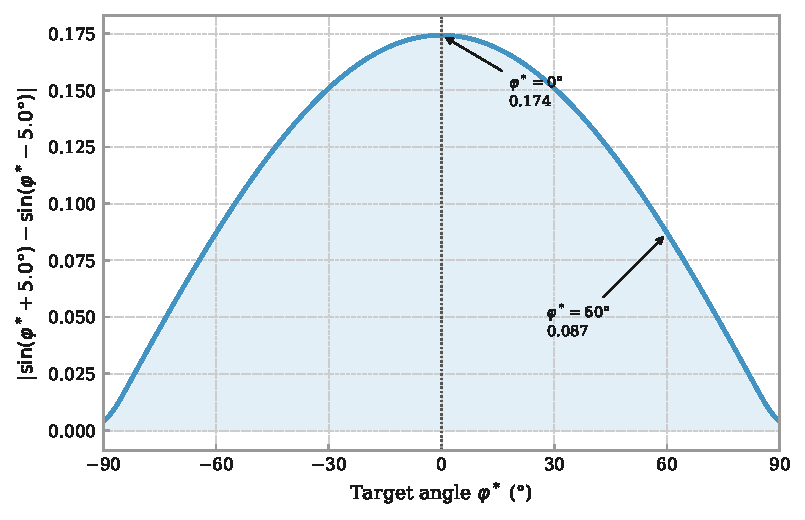
\includegraphics[width=0.75\textwidth]{images/chapter3/sampling_bandwidth.pdf}
    \caption{DDM constraint bandwidth in sin-space: broadside spans $0.174$ compared to $0.087$ at $60\degree$ resulting in a 2.0 ratio}
    \label{fig:sampling_constraint_bandwidth}
\end{figure}
\FloatBarrier

The matched-filter or\gls{DFT} steering vector, with phases $\psi_n = \pi\sin\varphi^* \cdot n$, is the canonical starting point for any beamformer: it maximises gain at $\varphi^*$ without imposing any further constraint. Under this choice, the array response phase increases linearly with $(\sin\varphi - \sin\varphi^*)$, giving a phase gradient at the target of:
\begin{equation}
    \frac{d\angle f}{d\varphi}\bigg|_{\varphi=\varphi^*} = \frac{N-1}{2}\,\pi\cos\varphi^*
\end{equation}
For $N = 5$ this evaluates to $2\pi\cos\varphi^*$ rad/rad, and the maximum phase deviation accumulated across the half-window $\delta\varphi$ is approximately:
\begin{equation}
    \Delta\angle f_{\max} \approx \frac{N-1}{2}\,\pi\cos\varphi^* \cdot \delta\varphi = 2\pi\cos\varphi^* \cdot \delta\varphi
\end{equation}
At broadside ($\varphi^* = 0\degree$, $\delta\varphi = 0.0873\,\text{rad}$) this gives $\Delta\angle f_{\max} \approx 31\degree$: more than three times the $\varepsilon_p = 10\degree$ tolerance. The crossover angle at which the\gls{DFT} solution just satisfies the phase constraint is:
\begin{equation}
    \varphi^*_{\text{cross}} = \arccos\!\left(\frac{\varepsilon_p}{\frac{N-1}{2}\pi\delta\varphi}\right) \approx 71\degree
\end{equation}
\figurename~\ref{fig:sampling_dft_deviation} confirms this threshold numerically: the\gls{DFT} deviation exceeds $\varepsilon_p$ for all $|\varphi^*| < 71\degree$, covering the entire range from $0\degree$ to $60\degree$. \figurename~\ref{fig:sampling_phase_curves} shows the detailed phase deviation curves for four representative target angles.
Since the\gls{DFT} solution maximises the inner product between the steering vector and the array manifold at $\varphi^*$, it is the attractor of any gradient ascent on received power, yet the valid broadside cluster sits elsewhere, separated from the\gls{DFT} solution by a broad infeasible region that provides no gradient bridge. The magnitude of this gap, a.k.a. how far the solution is from the valid cluster in steering vector space, grows as $\cos\varphi^*$ and is most severe at broadside.

\begin{figure}[htbp]
    \centering
    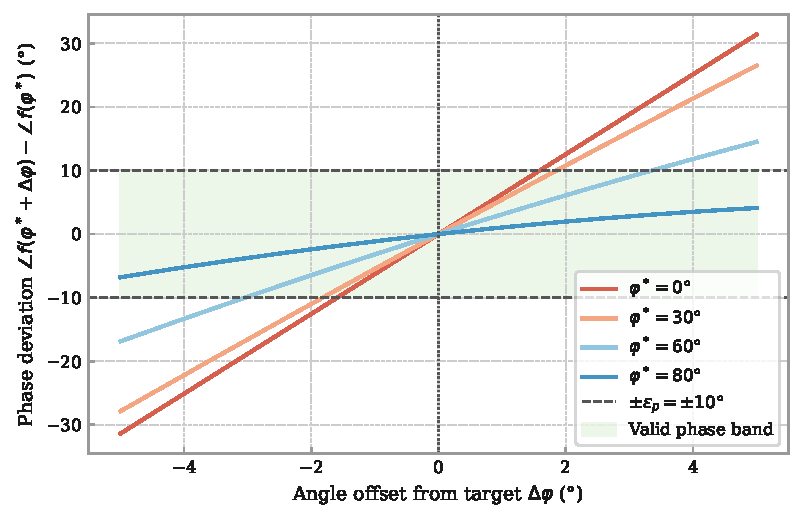
\includegraphics[width=0.75\textwidth]{images/chapter3/sampling_phase_curves.pdf}
    \caption{\gls{DFT} beamformer phase across $\pm5.0\degree$ window. Curves outside the green band require a non-\gls{DFT} solution.}
    \label{fig:sampling_phase_curves}
\end{figure}

\begin{figure}[htbp]
    \centering
    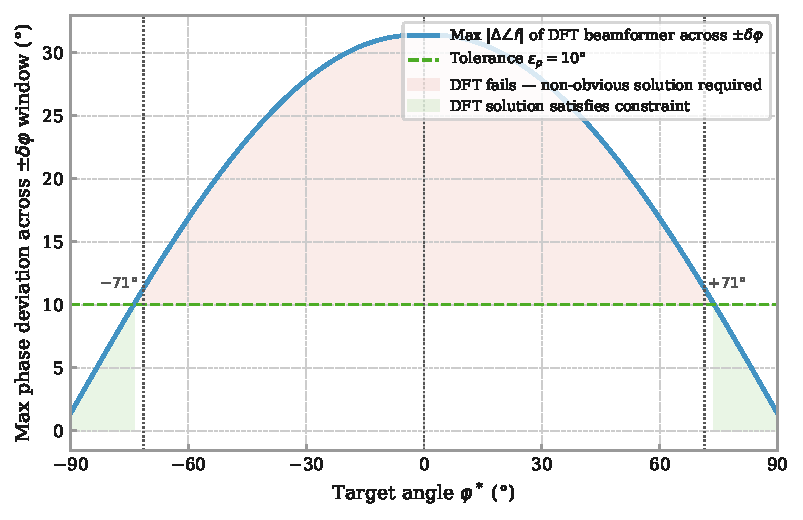
\includegraphics[width=0.75\textwidth]{images/chapter3/sampling_dft_deviation.pdf}
    \caption{\gls{DFT} beamformer phase deviation with N=5 elements. At broadside ($0\degree$): $31\degree$,\gls{DFT}-only solutions are valid only for $|\varphi^*| > 71\degree$}
    \label{fig:sampling_dft_deviation}
\end{figure}
\FloatBarrier

\subsubsection{The Sin-Space Sampling Bias}
\label{subsec:sin-space_sampling_bias}
The constraint difficulty described in \subsectionname~\ref{subsec:angle_dependant_constraint} is an intrinsic property of the\gls{ULA} geometry that can be exacerbated or alleviated by the chosen sampling strategy. 
Training angle sets are most naturally specified in degrees of azimuth: $\varphi \in \{-90\degree, -89\degree, \ldots, +90\degree\}$, a set of 181 angles uniformly spaced in $\varphi$. The Jacobian of the mapping $u = \sin\varphi$ is $du/d\varphi = \cos\varphi$, so equal angular steps $\Delta\varphi$ correspond to unequal $u$-space displacements:
\begin{equation}
    \Delta u \approx \cos\varphi^* \cdot \Delta\varphi
\end{equation}
Near broadside, ($\cos\varphi^* \approx 1$) each $1\degree$ step produces the largest possible displacement in $u$-space causing sampled angles to be spread across the broadside region while near endfire ($\cos\varphi^* \to 0$) the same angular step produces a negligible $u$-displacement causing large numbers of angles to crowd into a vanishingly narrow spatial-frequency band.
When $\varphi$ is drawn uniformly from $[-90\degree, 90\degree]$, the induced distribution of $u = \sin\varphi$ follows the arcsine law, $p(u) = 1/(\pi\sqrt{1-u^2})$, which diverges at $u = \pm 1$ and attains its minimum $1/\pi$ at $u = 0$. The histogram is therefore U-shaped: density is lowest at broadside and spikes sharply at the endfire limits, as shown by the blue histogram in \figurename~\ref{fig:sampling_density}. The red histogram shows the distribution obtained by sampling $u$ uniformly in $[-1, 1]$, flat by construction.
Concretely, with 181 uniform-in-$\varphi$ angles: the endfire neighbourhood $|\varphi| > 80\degree$ contributes 22 angles yet spans only ${\approx}3\%$ of the full $u$-domain. The broadside neighbourhood $|\varphi| < 10\degree$ contributes a comparable 21 angles but spans ${\approx}35\%$ of the $u$-domain, leaving it severely undersampled relative to its spatial-frequency extent.

\begin{figure}[htbp]
    \centering
    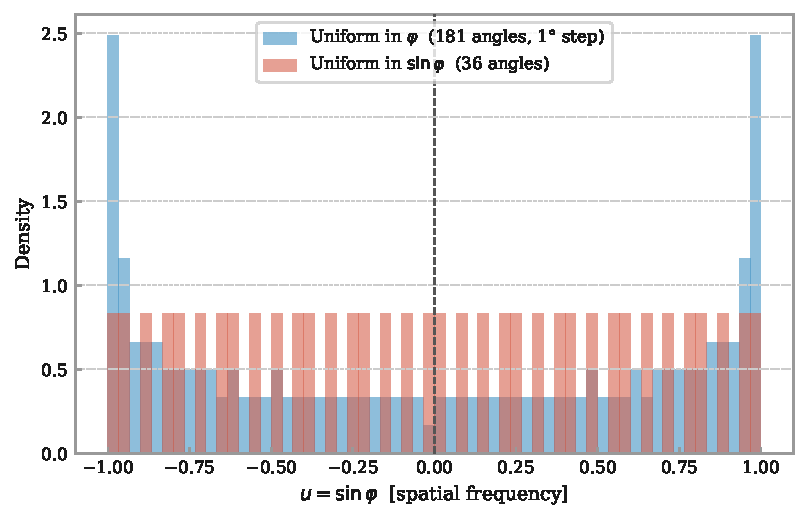
\includegraphics[width=0.75\textwidth]{images/chapter3/sampling_density.pdf}
    \caption{Angle density in sin-space. Sampling 181 angles with 1\degree step results in crowding in endfire while sin sampling results in a flat scheme.}
    \label{fig:sampling_density}
\end{figure}

\subsubsection{Compound Effect and Adopted Sampling Strategy}

The physical difficulty \subsectionname~\ref{subsec:angle_dependant_constraint} and the sampling bias \subsectionname~\ref{subsec:sin-space_sampling_bias} are independent mechanisms, but they can combine adversarially.
The physical difficulty means that each broadside episode is unlikely to yield a valid solution easily, so the policy needs many broadside episodes to accumulate enough successful exploration to converge on the valid cluster while the sampling bias simultaneously ensures that broadside receives the fewest episodes per unit of $u$-space: precisely the region that most needs a large exploration budget. Meanwhile, endfire receives the most episodes per $u$-space unit despite needing the least: the feasible set is large, the\gls{DFT} solution is already valid for $|\varphi^*| > 71\degree$, and the policy consolidates endfire performance quickly resulting in abundant valid rewards from endfire dominating the policy gradient leading to reinforcing strategies that work at endfire. These same strategies do not transfer to broadside as the valid solutions occupy a structurally different, concentrated cluster in steering vector space and because broadside episodes are infrequent, the corrective signal from broadside failures is too sparse to drive the policy toward the correct region.\\
Sampling training angles uniformly in $u = \sin\varphi$ and mapping back via $\varphi = \arcsin(u)$, produces the flat distribution shown in red in \figurename~\ref{fig:sampling_density}. This corrects the secondary cause: it equalises exploration budget across all spatial frequencies, shifting episodes away from the already mastered endfire region and toward the underexplored broadside region.
Addressing the physical difficulty, instead, requires an exploration regime capable of navigating a high-dimensional parameter space toward a geometrically concentrated feasible set and\gls{CL} provides a principled mechanism: the agent first builds intuition for what valid solutions look like at broadside angles, then transfers and refines that understanding as the constraint tightens and finally the target angles expand to the desired $[-90\degree, 90\degree]$.

\subsection{Training configuration}

\subsubsection{State Space}

The state space $\mathcal{S}$ encodes the target azimuth angle $\varphi$ together with the current constraint curriculum progress $\rho_c \in [0,1]$ (\subsubsectionname~\ref{subsubsec:curriculum_learning}). Rather than passing the raw angle in radians, the angular component is represented as its trigonometric projections:

\begin{equation}
    \mathbf{s} = \bigl[\cos(\varphi),\; \sin(\varphi),\; \rho_c\bigr] \in [-1, 1]^2 \times [0, 1]
\end{equation}
The trigonometric encoding keeps the angular components bounded in $[-1, 1]$ and preserves angular proximity in Euclidean distance. Including $\rho_c$ as a third observation component makes the environment \emph{stationary}: at any fixed pair $(\varphi,\,\rho_c)$ the optimal action and expected reward are fully determined, so the policy can condition its output on the current tightness of the physical constraints and avoid conflating loose early-curriculum episodes with tight late-curriculum episodes at the same target angle. The observation space is a bounded continuous box $\mathcal{S} \subseteq [-1,1]^2 \times [0,1]$, with all three components of type \texttt{float32}.

\subsubsection{Action Space}
The action space $\mathcal{A}$ is a continuous box of dimension $2N$ where $N$ is the number of antenna elements in the\gls{ULA}. Each action vector is split into two equal halves:

\begin{equation}
    \mathbf{a} = [\underbrace{a_1, \dots, a_N}_{\text{phase}},\;
    \underbrace{a_{N+1}, \dots, a_{2N}}_{\text{amplitude}}] \in [-1, 1]^{2N}
\end{equation}
All components are normalized to the interval $[-1, 1]$ as required by the\gls{PPO} policy network. At inference time, the two halves are rescaled into their physical ranges. The phase components are mapped to $[0, 2\pi]$:

\begin{equation}
    \varphi_n = a_n \cdot \pi + \pi, \quad n = 1, \dots, N
\end{equation}

and the amplitude components are mapped to $[0, 1]$:

\begin{equation}
    \alpha_n = a_{N+n} \cdot 0.5 + 0.5, \quad n = 1, \dots, N
\end{equation}
This symmetric normalization keeps the action distribution centered around zero, which is beneficial for the stability of gradient-based policy optimization.
\begin{figure}[htbp]
    \centering
    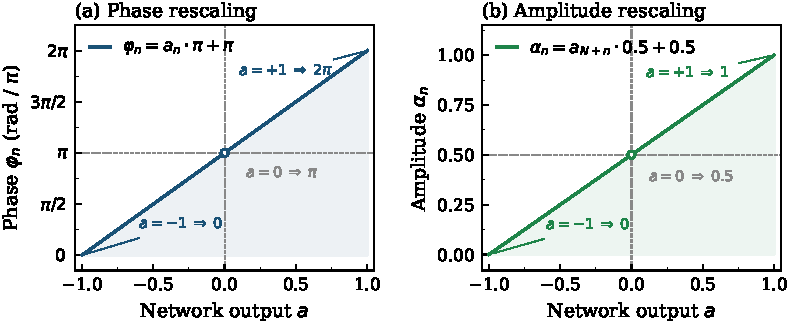
\includegraphics[width=0.75\textwidth]{images/chapter3/network_output_mapping.pdf}
    \caption{Phase and amplitude mapping}
    \label{fig:network_output_mapping}
\end{figure}
\FloatBarrier
An alternative physics-informed residual parameterisation, in which the action encodes corrections to the\gls{DFT} steering vector rather than absolute phases, is evaluated in \subsectionname~\ref{subsec:physics_informed} and visualized in \figurename~\ref{fig:physics_informed_network_output_mapping}.
\begin{figure}[htbp]
    \centering
    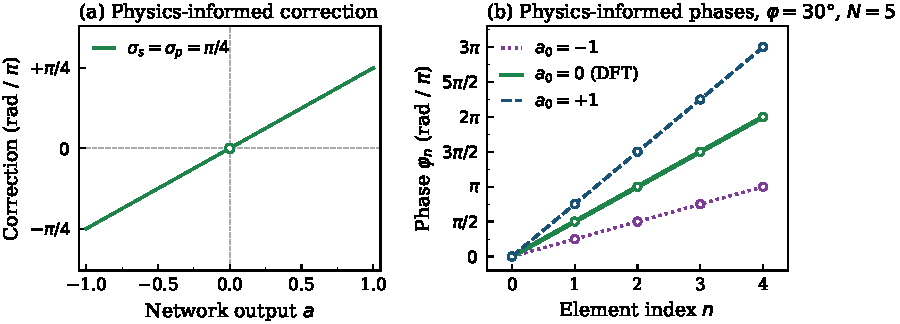
\includegraphics[width=0.75\textwidth]{images/chapter3/physics_informed_mapping.pdf}
    \caption{Phase physics informed mapping}
    \label{fig:physics_informed_network_output_mapping}
\end{figure}

\subsubsection{Transition Function}

The environment is formulated as a \textit{contextual bandit}, meaning that every episode consists of exactly one interaction step; At the beginning of each episode, a target angle $\varphi$ is sampled uniformly at random from the discrete set of training angles $\varphi_{\text{train}}$:

\begin{equation}
    \varphi \sim \mathcal{U}(\varphi_{\text{train}})
\end{equation}
The agent observes the encoding $\mathbf{s} = [\cos\varphi, \sin\varphi, \rho_c]$, produces a single action $\mathbf{a}$, receives a scalar reward $r$, and the episode terminates immediately with \texttt{terminated = True}. There is no temporal state transition; the next state is irrelevant, since the episode ends after each step.\\
This bandit formulation is a deliberate and central architectural choice: the optimal beamforming configuration for a given $\varphi$ is stateless since it does not depend on any history of prior actions, and there is no sequential decision process to unroll. Casting the problem as a bandit therefore removes a layer of complexity that would otherwise be artificial, eliminates the credit assignment problem across time steps, and allows the agent to receive an immediate and unambiguous reward signal for every configuration it proposes. \\
Generalization across angles is achieved by randomizing $\varphi$ at each reset, forcing the policy to learn a direct mapping from angle encoding to beamforming configuration rather than momorizing a fixed solution for a single direction.
\subsubsection{Reward Function}
The reward signal $r$ is a composite of four tiers designed to guide the agent progressively from geometrically valid beam shapes toward configurations that jointly maximise the\gls{BER} performance of the legitimate receiver and the decoding difficulty for potential eavesdroppers. The design directly optimises communication and\gls{PLS} metrics rather than relying on beam geometry alone to imply them.

\subsubsection{Amplitude coherence terms.}
Before the soft constraint evaluation, two amplitude terms provide a base gradient over the element weights $\boldsymbol{\alpha} = [\alpha_1, \ldots, \alpha_N]^\top$:
\begin{equation}
    r_{\text{amp}} = 20\,\overline{\alpha} + 7\,\overline{\log\max(\alpha_n,\,0.01)}
\end{equation}
where $\overline{\alpha} = \frac{1}{N}\sum_n \alpha_n$ is the mean amplitude and the log term is the per-element mean of $\log(\alpha_n)$ clamped at $10^{-2}$. The linear term pushes all elements toward full power, while the log penalty imposes a large gradient near zero and discourages any element from being completely silenced. The clamp at $10^{-2}$ bounds the penalty at $\approx -6.5$ per element so the gradient does not vanish for fully-off elements.

\subsubsection{Soft constraint terms.}
The second tier evaluates the soft\gls{DDM} validity of the produced steering vector. Four statistics are extracted from the soft validation function evaluated over a 2D grid of $N_v = 40$ points per axis (a $40 \times 40$ grid within the support $[\theta_{\mathrm{ref}} \pm \delta_\theta] \times [\varphi \pm \delta_\varphi]$): the mean amplitude score $s_a \in [0,1]$, the mean phase score $s_p \in [0,1]$, the minimum phase sigmoid $p_{\min} \in [0,1]$, and the mean absolute phase deviation $\bar{\delta\varphi}$. The soft constraint reward is:
\begin{equation}
    r_{\text{val}} = 3\,s_a + 4\,s_p + p_{\min} - 2\,\frac{\bar{\delta\varphi}}{\pi}
\end{equation}
The four terms are additive, so each provides an independent gradient signal throughout training; Positive terms reward progress toward the feasible region even before full validity is achieved, while the penalty on $\bar{\delta\varphi}$ discourages large average phase errors that keep the gradient alive when the policy is far from the validation constraints.

\subsubsection{Legitimate receiver BER.}
The third tier directly optimises the\gls{BER} experienced by the intended receiver. Given the normalized array gain $|f^*|$ at the target direction and the curriculum-adjusted reference\gls{SNR} $\mathrm{SNR}_0$ (\subsubsectionname~\ref{subsubsec:curriculum_learning}), the received $E_s/N_0$ is $|f^*|^2 \cdot 10^{\mathrm{SNR}_0/10}$ and the theoretical $M$-\gls{PSK}\gls{BER} (with $M = 8$ throughout this work) is:
\begin{equation}
    B_{\text{legit}} = \mathrm{BER}_{M\text{-PSK}}\!\left(|f^*|^2 \cdot 10^{\mathrm{SNR}_0/10}\right)
\end{equation}
A log-scale\gls{BER} score maps this to a normalised reward in $[0, 1]$:
\begin{equation}
    \mathrm{BER\_score} = \frac{\log_{10} B_{\text{legit}} - \log_{10} 0.5}{\log_{10} B_{\text{target}} - \log_{10} 0.5}
\end{equation}
where $B_{\text{target}} = 10^{-4}$. The score equals $1$ when $B_{\text{legit}} \leq B_{\text{target}}$ (performance target met) and $0$ when $B_{\text{legit}} = 0.5$ (random guessing), providing a dense gradient over the full range of array gain. The\gls{BER} reward is:
\begin{equation}
    r_{\text{ber}} = w_{\text{ber}} \cdot \mathrm{BER\_score}, \quad w_{\text{ber}} = 5
\end{equation}
This term is applied unconditionally, without gating on validity, since amplitude coherence that increases array gain simultaneously improves the soft constraint scores, making a gate unnecessary and harmful to gradient flow.

\subsubsection{Pre-validation secrecy incentive.}
The fourth pre-validation term rewards configurations that produce high\gls{BER} at eavesdropper positions. For each angle $\varphi_e$ in the training set satisfying $|\varphi_e - \varphi| > 10^\circ$, the eavesdropper\gls{BER} is computed accounting for both the received\gls{SNR} and the phase offset relative to the legitimate receiver:
\begin{equation}
    B_e(\varphi_e) = \mathrm{BER}_{M\text{-PSK}}\!\left(|f(\varphi_e)|^2 \cdot 10^{\mathrm{SNR}_0/10},\; \angle f(\varphi_e) - \angle f^*\right)
\end{equation}
The phase-aware\gls{BER} formula accounts for the fact that a phase error of $\pi/M$ places the received symbol on a decision boundary, maximising decoding errors regardless of\gls{SNR}. The unweighted mean eavesdropper\gls{BER} $\bar{B}_e$ (every eavesdropper angle counted equally, so that low-amplitude sidelobe angles receive the same gradient signal as main-beam directions) defines the secrecy\gls{BER} gap:
\begin{equation}
    \Delta B = \bar{B}_e - B_{\text{legit}} \in [-0.5,\; 0.5]
\end{equation}
A positive gap indicates that eavesdroppers on average experience a higher error rate than the legitimate receiver. The pre-validation secrecy reward is:
\begin{equation}
    r_{\text{sec}} = 5\,\max(0,\, \Delta B)
\end{equation}
Only positive gaps are rewarded before validity is confirmed, so early exploration is not penalised for failing to achieve secrecy before the beam shape itself is geometrically valid.

\subsubsection{Validity bonus and secrecy penalties.}
When the hard validity check passes, a structured validity bonus reinforces secrecy objectives:
\begin{equation}
    r_{\text{valid}} = w_\varphi \cdot 20 + 25\,\Delta B + w_{\text{wc}} \cdot \Delta B_{\min} - 35\,f_{\text{low}} + 15\,|f^*|
\end{equation}
where:
\begin{itemize}
    \item $w_\varphi = 1 + |\cos\varphi| \in [1, 2]$ is an angle-dependent weight that assigns double credit to broadside solutions, compensating for the structural difficulty at $\varphi \approx 0^\circ$ described in \subsectionname~\ref{subsec:angle_dependant_constraint}.
    \item $\Delta B_{\min} = B_{e,\min} - B_{\text{legit}}$ is the worst-case secrecy gap, where $B_{e,\min}$ is the minimum\gls{BER} across all eavesdropper angles (the easiest-to-decode adversary). The weight is $w_{\text{wc}} = 80$ if $\Delta B_{\min} < 0$ and $w_{\text{wc}} = 50$ otherwise, imposing a stronger penalty when the worst-case eavesdropper outperforms the legitimate receiver.
    \item $f_{\text{low}}$ is the fraction of eavesdropper angles with $B_e < 0.1$, penalising solutions that leave a large proportion of the angular space trivially decodable.
    \item The $15|f^*|$ term provides a gradient, pushing the array gain above the constraint floor toward maximum coherent gain; the\gls{BER} score saturates at $w_{\text{ber}}$ for any valid configuration at training\gls{SNR}, making this term the sole remaining gradient for increasing gain once validity is achieved.
\end{itemize}

\subsubsection{Total reward}
The total reward is:
\begin{equation}
    r = r_{\text{amp}} + r_{\text{val}} + r_{\text{ber}} + r_{\text{sec}} + \mathbf{1}[\text{valid}]\cdot r_{\text{valid}}
\end{equation}
with any non-finite value replaced by $r = -1$ to guard against numerical instability. The four pre-validation tiers provide dense gradient signals throughout training; the validity-gated tier provides the long-horizon objective that can only be earned by configurations that are simultaneously geometrically valid and secrecy-aware.


\subsubsection{Curriculum Learning}
\label{subsubsec:curriculum_learning}
Training a policy directly against the final, tightest physical constraints and the full angular range from the first iteration is inefficient as shown in \subsectionname\ref{subsec:curriculum_flattened}: the feasible region is small, the\gls{BER} and secrecy rewards are rarely triggered, and the reward landscape is nearly flat for most of the early training budget. A structured curriculum therefore progressively tightens the constraints and expands the range of training angles as training advances \cite{bengio2009curriculum}. Two independent progress scalars govern the curriculum:
\begin{equation}
    \rho_c = \min\!\left(\frac{t}{T \cdot r_c},\, 1\right), \qquad
    \rho = \min\!\left(\frac{t}{T \cdot r_s},\, 1\right)
\end{equation}
where $T$ is the total training budget, $r_c = 0.12$ is the constraint curriculum ratio (constraints reach their final values at $12\%$ of $T$), and $r_s = 0.20$ is the angle expansion ratio (the full angular range is unlocked at $20\%$ of $T$). The constraint progress $\rho_c$ is also included as the third observation component, making the environment stationary across curriculum stages.

\subsubsection{Amplitude tolerance $\epsilon_a$.}
The amplitude floor is annealed as:
\begin{equation}
    \epsilon_a(\rho_c) = -6 + 5.3\,\rho_c
\end{equation}
At $\rho_c = 0$ the floor sits at $-6$, imposing $|f| \geq 10^{-6} \approx 0$ that means effectively no amplitude constraint. By $\rho_c = 1$ it has risen to $-0.7$, requiring $|f| \geq 10^{-0.7} \approx 0.20$ everywhere in the window.

\subsubsection{Phase tolerance $\epsilon_p$.}
The maximum allowable phase deviation is tightened monotonically:
\begin{equation}
    \epsilon_p(\rho_c) = 30^\circ - 20^\circ \cdot \rho_c
\end{equation}
The agent begins with a generous $30^\circ$ phase margin, which accepts a wide range of steering vectors, and converges to a strict $10^\circ$ tolerance by the end of the constraint curriculum.

\subsubsection{Reference SNR.}
The reference transmit\gls{SNR} used for\gls{BER} reward evaluation is also annealed:
\begin{equation}
    \mathrm{SNR}_0(\rho_c) = 20\,\text{dB} - 3\,\text{dB} \cdot \rho_c
\end{equation}
Starting at $20\,\text{dB}$ provides a strong, unambiguous\gls{BER} gradient early in training. The\gls{SNR} decreases to $17\,\text{dB}$ by the end of the constraint curriculum, tightening the performance target as the beam quality requirement tightens simultaneously.

\subsubsection{Angle range curriculum.}
Before angle expansion begins (first $7\%$ of timesteps), the agent trains exclusively on broadside-adjacent angles $|\varphi| \leq 10^\circ$, where the\gls{DDM} feasibility problem is most constrained. The reachable training angle range then expands linearly from $\pm 10^\circ$ to $\pm 90^\circ$ between $7\%$ and $20\%$ of total timesteps:
\begin{equation}
    \varphi_{\max}(t) =
    \begin{cases}
        10^\circ & t < 0.07\,T \\[4pt]
        10^\circ + 80^\circ \cdot \dfrac{t/T - 0.07}{0.13} & 0.07\,T \leq t < 0.20\,T \\[4pt]
        90^\circ & t \geq 0.20\,T
    \end{cases}
\end{equation}
This staged expansion ensures the policy first builds valid broadside solutions before being exposed to the easier endfire angles, which would otherwise dominate the policy gradient.

\subsubsection{Broadside-biased sampling.}
During the expansion phase, sampling is biased toward the broadside region $|\varphi| \leq 30^\circ$ (region A) over the wider angular range (region B) through three equal-duration stages:
\begin{center}
\begin{tabular}{cccc}
\hline
Stage & Timestep range & $P(\text{region A})$ & $P(\text{region A})$ \\
\hline
1 & $[\phantom{0}7\%,\; 38\%]\,T$ & $80\%$ & $20\%$ \\
2 & $[38\%,\; 69\%]\,T$ & $60\%$ & $40\%$ \\
3 & $[69\%,\; 100\%]\,T$ & $50\%$ & $50\%$ \\
\hline
\end{tabular}
\end{center}
The three stages divide the period from expansion start to end of training into three equal thirds, each spanning $31\%$ of $T$. The reduction from $80\%$ to $50\%$ is deliberately slow: broadside solutions remain structurally harder than endfire solutions even after the angle range is fully open, so a sustained bias toward $|\varphi| \leq 30^\circ$ continues to provide corrective gradient throughout training. The final $50/50$ split preserves balance without starving any part of the angular range. \figurename~\ref{fig:curriculum_overview} summarises all four curriculum dimensions on a shared time axis, with the four training phases indicated by background shading.

\begin{figure}[htbp]
    \centering
    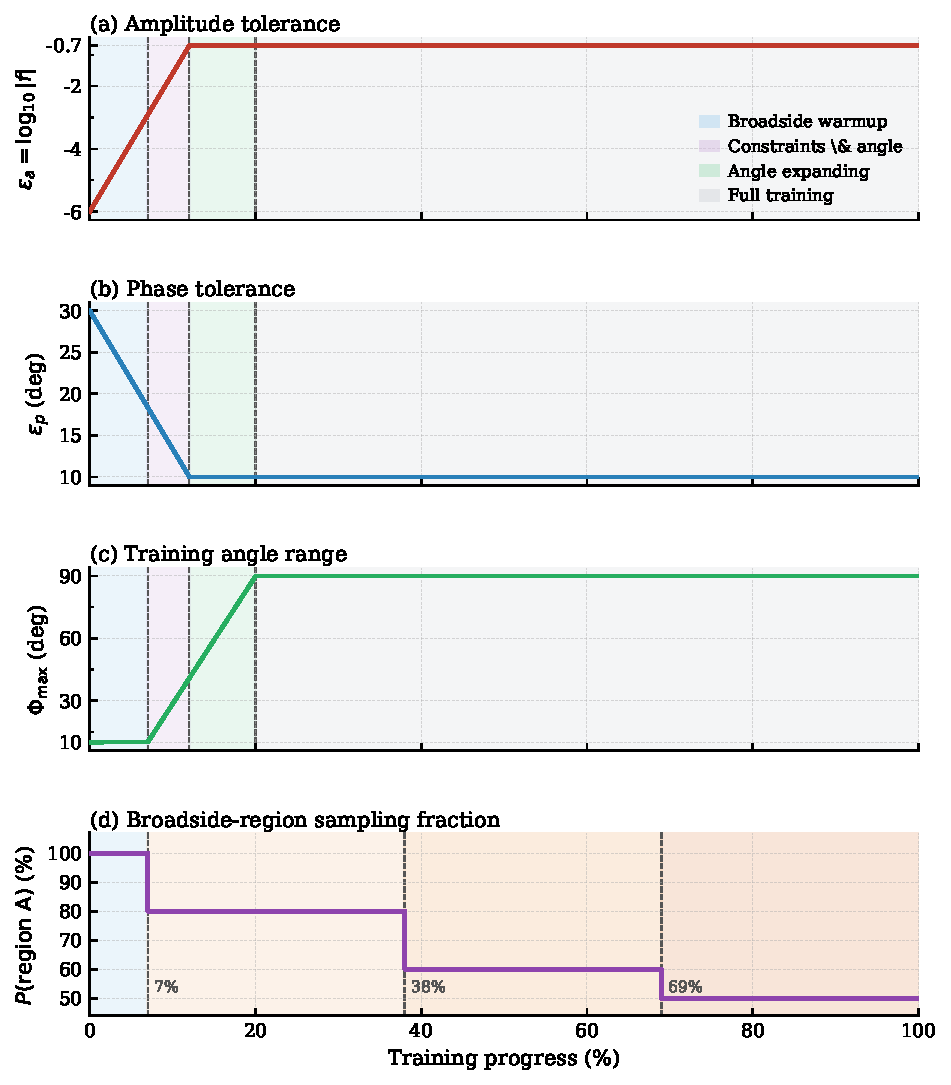
\includegraphics[width=0.85\textwidth]{images/chapter3/curriculum_overview.pdf}
    \caption{Complete curriculum schedule over training. Panel (a): amplitude floor $\varepsilon_a = \log_{10}|f|$ (raw base-10 logarithm of the normalised amplitude, not standard dB), rising from $-6$ ($|f| \geq 10^{-6} \approx 0$) to $-0.7$ ($|f| \geq 0.20$, or $-14\,\text{dB}$ standard). Panel (b): phase tolerance $\varepsilon_p$, from $30^\circ$ to $10^\circ$. Panels (a) and (b) complete at $12\%$ of total timesteps. Panel (c): training angle range, expanding from $\pm 10^\circ$ to $\pm 90^\circ$ between $7\%$ and $20\%$. Panel (d): broadside-region sampling fraction. Background shading marks the four phases: broadside warmup (blue, $0$--$7\%$), overlap (purple, $7$--$12\%$), angle-only expansion (green, $12$--$20\%$), and full training (grey, $20$--$100\%$). Dashed vertical lines mark transitions at $7\%$, $12\%$, and $20\%$; panel (d) uses orange shades for the three sampling stages ($7$--$38\%$, $38$--$69\%$, $69$--$100\%$).}
    \label{fig:curriculum_overview}
\end{figure}